\documentclass{article}
\usepackage{graphicx} % Required for inserting images
\usepackage{amsmath} 
\usepackage{float}
\usepackage{listings}

\newcommand{\probP}{\text{I\kern-0.15em P}}
\newcommand {\sig}{(1 + e^{-\theta^Tx_{i}})}

\title{Assign-3}
\author{Surendra Parla}
\date{February 2024}

\begin{document}

\maketitle

\section{1}
\subsection{a}
% \begin{text}
 Start with a large learning rate like 1 and 0.1. We could see that log-likelihood is quite unstable (highly fluctuating) which points out that we are just alternating on either side and not converging. 
 \begin{figure}[hp]
  % \centering
  % \begin{picture}(4,4)  % Replace with desired width and height
    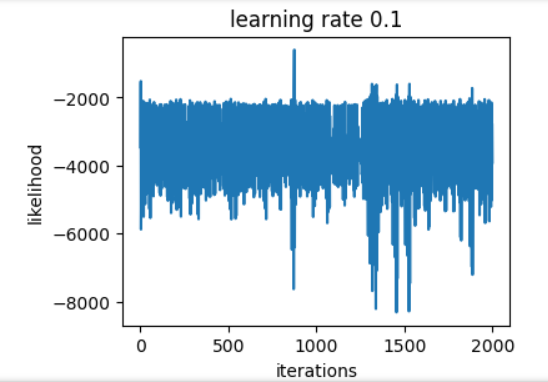
\includegraphics[width=10cm, height=6cm]{image.png}
    % \put(x,y){\captionof{figure}{My image caption}}  % Replace x,y with desired caption placement
  % \end{picture}
\end{figure}
    
Now, start 0.1 and for each iteration increase alpha increases linearly in the exponential space (0.1 to 0.0001) and plot the likelihood function.

 % \begin{figure}
  % \centering
  % \begin{picture}(4,4)  % Replace with desired width and height
    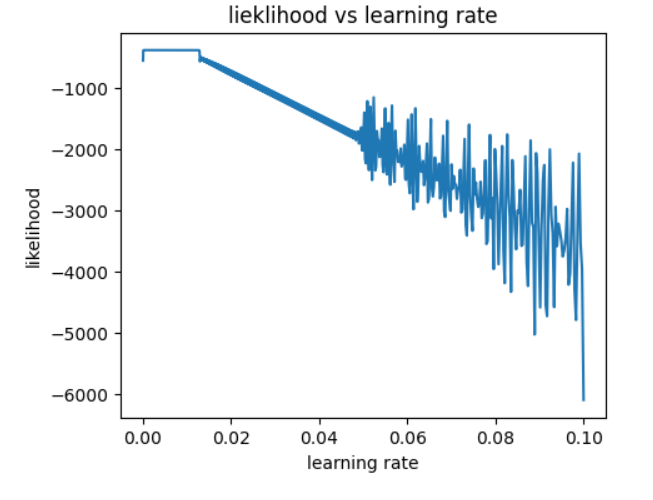
\includegraphics[width=10cm]{3-2.png}
    % \put(x,y){\captionof{figure}{My image caption}}  % Replace x,y with desired caption placement
  % \end{picture}
% \end{figure}

From the plot we can see there are 3 phases, when alpha is between 0 and 0.02 the training is so slow and if alpha is between 0.05 and 0.1 training is very unstable. So we can choose alpha as 0.001 for first few iterations and in final stages of training we can decrease it to 0.0001

As, the dataset is small learning rate of 0.001 worked significantly well

\subsection{b}
With proper normalization, the model converged in 30 iterations

\subsection{c}
Final value of $\hat{\theta}$ is [-0.88150697,  1.35276923, -0.56007237, -0.37063885, -0.13861887,0.23049696]

\subsection{d}
Maximum likelihood l($\theta$) is -374.6

\subsection{e}
The asymptotic distribution of $\theta$ is a normal distribution with mean $\hat{\theta}$ \\
{[-0.88150697,  1.35276923, -0.56007237, -0.37063885, -0.13861887,0.23049696] }\\
variance: \\
$
\begin{pmatrix}
78.82548935 &  4.88108223 &  15.71643104 &  18.15891713 & -29.45507336 & 144.69437922 \\
4.88108223 &   3.35126473 &   7.077103  &   6.40572294 & 3.94964209 &  -2.42939071 \\
15.71643104 &   7.077103  &  46.21584323 &  29.31906738 & 16.17231909 & -23.0911871 \\
18.15891713 &   6.40572294 &  29.31906738 &  31.3669466 & 9.52833911 &  -7.46410436 \\
-29.45507336 &   3.94964209 &  16.17231909 &   9.52833911 & 38.07379323 & -93.99912166 \\
144.69437922 &  -2.42939071 & -23.0911871 &  -7.46410436 & -93.99912166 & 350.71045394 
\end{pmatrix}
$

\section{2}
\subsection{a}
log odds \\
\begin{align*}
    \omega^\star = \log \frac{\probP(y = 1 | x)}{\probP(y = 0 | x)} &= \frac{\frac{1}{\sig}}{\frac{1}{(1 + e^{\theta^Tx)}}} \\
    &= \frac{(1 + e^{\theta^Tx)}}{(1 + e^{-\theta^Tx)}}  \\
 &= {\theta^\star}^TX
\end{align*}

where ${\theta^\star}^T$ is {[-0.88150697,  1.35276923, -0.56007237, -0.37063885, -0.13861887,0.23049696] } and X is the new sample \\
\begin{math}
    variance = Var({\theta^\star}^TX) = X^TVar({\theta^\star}^T)X  = X^TI^{-1}_{\theta^*}X
\end{math}
\section{3}
\subsection{a}
Lets assume I am on the titanic my feature vector would be 
X = 
$
\begin{pmatrix}
    2 \\
    0 \\
    25 \\
    0 \\
    0 \\
    20
\end{pmatrix} \\
$
${Y_{new} \left( \text{probability of survival is 0.42179714} \right) \text{is 0.}} $\\
\text{So, I would have been deceased in the titanic.}
\subsection{b}
\text{Variance is $X_{new}^TI_{\theta^*}^{-1}X$} = 85.73272155 \\
$\sigma = 9.25919659$ \\
$\tau = 1.96*\sigma/\sqrt{800}$ \\
$\tau = 0.72949679$ \\ 
\subsection{c}
$\hat{\omega} = \theta^TX = -0.31540031$ \\
\text{Interval for log-odds is (-0.31540031 $\pm$ 0.72949679)} \\
\text{So, odds are in the interval [0.36787944, 1.4918247] which shows that we may or may not have survived.}
\section{4}
\subsection{a}
\begin{equation}
\text{With } p\text{-value} = \Phi_{\chi^2}\left(\frac{\widehat{\theta}_j^2}{\nu_j^2}\right) \text{ we conclude that the } j^\text{th} \text{ feature is significant if $\widehat{\theta}_j^2 > \nu_j^2 \Phi_{\chi^2}^{-1}(\alpha)$}
\end{equation}

\subsection{b}
$\nu_j^2$ = $
\begin{pmatrix}
78.82548 &  3.35126 & 46.21584 & 31.36694 & 38.07379 & 350.71045
 \end{pmatrix} $
 \\
$\widehat{\theta}_j^2$ = $
\begin{pmatrix}
0.77705454 & 1.82998458 & 0.31368106 & 0.13737316 & 0.01921519 & 0.05312885
 \end{pmatrix} $
$\left(\frac{\widehat{\theta}_j^2}{\nu_j^2}\right)$ = $
\begin{pmatrix}
9.85790955e-03 \\ 5.46057899e-01 \\  6.78730574e-03 \\ 4.37955151e-03 \\
5.04682851e-04 \\ 1.51489203e-04
\end{pmatrix}
$
$\Phi_{\chi^2}^{-1}(\alpha)$ = 0.00393 for 1 dof and 95\% significance

Therefore features Pclass, Sex, Age, Siblings/Spouses Aboard are significant and 
features Parents/Children Aboard and Fare are insignificant 

\subsection{c}
Sex is the most significant feature.  \\ 
So, changing the feature and calculating the $Y_{new} \left(we get probability 0.5262661\right)$ = 1. \\
I would have survived if we change the significant feature.

\section{Appendix}
Accuracy by 90:10 split is around 80\%. \\
\begin{lstlisting}
split_ratio = 0.9
num_samples = df.shape[0]
num_train = int(num_samples * split_ratio)
num_test = num_samples - num_train
y = df.iloc[:, 0].astype(np.int32).to_numpy()
Y_train, Y_test = y[:num_train], y[num_train:]
x = df.iloc[:, 1:7].astype(np.float64).to_numpy().T
X_train, X_test = x[:,:num_train], x[:,num_train:]
mean = X_train.mean(axis=1).reshape([6,1])
std = X_train.std(axis=1).reshape([6,1])
X_train, X_test = (X_train-mean)/std, (X_test-mean)/std

def sigmoid(x):
  return 1 / (1 + np.exp(-x))

def find_likelihood(theta, x, y):
    likelihood = 0
    for i in range(len(y)):
        if y[i] == 1:
            likelihood += np.log(sigmoid(np.matmul(theta, x[:,i])))
        else:
            likelihood += np.log(sigmoid(-np.matmul(theta, x[:,i])))
    return likelihood

theta_list = []
likelihood_list = []
iter = 1000
# alpha = 10**np.linspace(-3,-1,500)
def train(x,y, theta, iter):
    for i in range(iter):
        y_hat = sigmoid(np.matmul(theta, x))
        # print(y_hat)
        grad = np.sum(x*(y-y_hat), axis=1)
        # grad_list.append(grad)
        # print(grad)
        alpha = 0.001 if i < 30 else 0.0001
        
        theta = theta + alpha*grad
        theta_list.append(theta)
        # print(theta)
        
        likelihood = find_likelihood(theta, x, y)
        likelihood_list.append(likelihood)
train(X_train, Y_train,theta, iter)

plt.figure(figsize=(15,4))
plt.xlabel('iterations')
plt.ylabel('likelihood')
plt.title('lieklihood vs learning rate')
plt.plot(likelihood_list)
plt.show()

def predict(x,y, theta):     
    y_hat = sigmoid(np.matmul(theta, x))
    y_pred = list(map(lambda l: 1 if l>=0.5 else 0, y_hat))
    print(y_pred)
    count = 0
    for i in range(len(y)):
        if y[i] == y_pred[i]:
            count += 1
    print('accuracy', count/len(y))
    return count/len(y)

#information matrix
def expo(x):
    return np.exp(-x)/(1+np.exp(-x))**2

def information_matrix(x, theta):
    info = np.zeros((x.shape[0], x.shape[0]))
    for i in range(len(x)):
        info += expo(theta@x[:, i])*(x[:, i].reshape(-1, 1)@x[:, i].reshape(-1, 1).T)
    return info
infomat = information_matrix(X_train, theta_star)
infomat_inv = np.linalg.inv(infomat)
\end{lstlisting}
\end{document}
